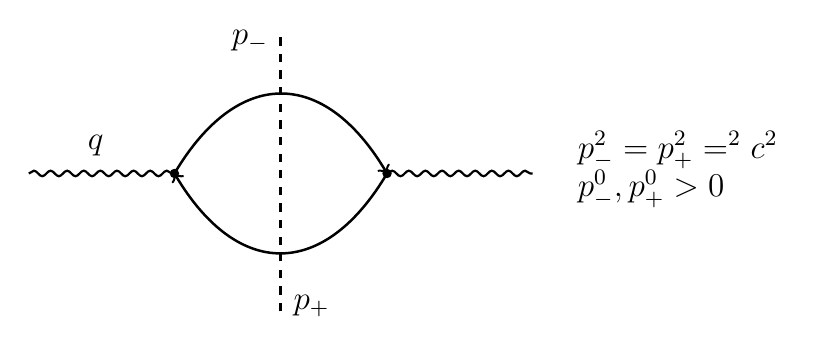
\begin{tikzpicture}[x=1cm,y=1cm,every node/.style={font=\large}]
 \coordinate (L) at (-3.2,0); \coordinate (a) at (-1.35,0);
 \coordinate (b) at (1.35,0); \coordinate (R) at (3.2,0);
 \draw[decorate,decoration={snake,amplitude=1.0pt,segment length=6pt},line width=.8pt] (L)--(a);
 \draw[decorate,decoration={snake,amplitude=1.0pt,segment length=6pt},line width=.8pt] (b)--(R);
 \draw[->,line width=.9pt] (a) .. controls (-.55,1.35) and (.55,1.35) .. (b);
 \draw[->,line width=.9pt] (b) .. controls (.55,-1.35) and (-.55,-1.35) .. (a);
 \fill (a) circle (1.7pt); \fill (b) circle (1.7pt);
 \draw[dashed,line width=1.05pt] (0,-1.75)--(0,1.75);
 \node at (-2.35,.35) {$q$};
 \node[anchor=south east,fill=white,inner sep=1pt] at (-.12,1.50) {$p_-$};
 \node[anchor=north west,fill=white,inner sep=1pt] at (.12,-1.50) {$p_+$};
 \node[align=left,right] at (3.65,.05) {$p_-^2=p_+^2=\me^2c^2$\\$p_-^0,p_+^0>0$};
\end{tikzpicture}
